%
% teil1.tex -- Beispiel-File für das Paper
%
% (c) 2020 Prof Dr Andreas Müller, Hochschule Rapperswil
%
% !TEX root = ../../buch.tex
% !TEX encoding = UTF-8
%
\section{Das Katenoid
	\label{minimalflaechen:section:Das Katenoid}}
\rhead{Das Katenoid}
Da im Kapitel \ref{chapter:kettenlinie} bereits die Kettenlinie behandelt wurde, wird hier das Katenoid als Erweiterung der Erkenntnisse über die Kettenlinie näher erläutert. 

\subsection{Katenoid und Kettenlinie
	\label{Das Katenoid:subsection:Katenoid und Kettenlinie}}
Die Form eines Katenoids kann durch die Lösung der Euler-Lagrange-Gleichung für Minimalflächen bestimmt werden.
Diese Gleichung ergibt sich aus der Bedingung, dass die erste Variation des Flächeninhalts null ist.
Die Euler-Lagrange-Gleichung lautet
\begin{equation}
	\frac{\partial L}{\partial y} - \frac{d}{dx} \frac{\partial L}{\partial y'} = 0.
\end{equation}
%
Die Lösung dieser Gleichung ergibt die bekannte Gleichung der Kettenlinie
\begin{equation}
	y(x) = a \cdot \cosh \left( \frac{x - x_0}{a} \right) + y_0,
\end{equation}
%
wobei
\begin{itemize}
	\item \(a\) = Krümmungsradius im Scheitelpunkt,
	\item \(x_0\) = Verschiebung in $x$-Richtung,
	\item \(y_0\) = Verschiebung in $y$-Richtung
\end{itemize}
bedeutet.

Diese Gleichung beschreibt die Form der Kettenlinie, die durch die Schwerkraft beeinflusst wird und eine Minimalfläche bildet.
Für eine detaillierte Berechnung siehe Kapitel \ref{chapter:kettenlinie}.
\subsection{Katenoid als minimale Rotationsfläche
	\label{Das Katenoid:subsection:Katenoid als minimale Rotationsfläche}}
Mit den folgenden Schritten werden wir überprüfen, ob die Funktion  \( y(x) = a \cdot \cosh \left( \frac{x}{a} \right) \) der Euler-Lagrange DGL genügt und somit die Bedingung für Minimalflächen erfüllt ist.
Zuerst brauchen wir das Flächenintegral der Rotationsfläche, die durch die Drehung einer Kurve um die $x$-Achse entsteht:
\begin{equation}
	A = 2\pi \int_{a}^{b} y(x) \sqrt{1 + (y'(x))^2} \,dx.
\end{equation}
Somit lautet die Lagrange-Funktion 
\begin{equation}
	L(x, y, y') = y \sqrt{1 + (y')^2}.	
\end{equation}
Folgende Bedingung muss erfüllt sein: 
\begin{equation}
	\frac{\partial L}{\partial y} - \frac{d}{dx}  \frac{\partial L}{\partial y'} = 0.
\end{equation}
An dieser Stelle brauchen wir die partiellen Ableitungen

\begin{equation}
	\frac{\partial L}{\partial y} = \sqrt{1 + (y')^2}
\end{equation}
und 
\begin{equation}
	\frac{\partial L}{\partial y'} = y \frac{y'}{\sqrt{1 + (y')^2}}.
\end{equation}
Damit es sich um eine Minimalfläche handelt, muss die Gleichung
\begin{equation}
	\sqrt{1 + (y')^2} = \frac{d}{dx} \left( y \frac{y'}{\sqrt{1 + (y')^2}} \right)
	\label{minimalflaechen:eqn:elgleichung}
\end{equation}
erfüllt sein.
Wenn wir in der Gleichung \eqref{minimalflaechen:eqn:elgleichung}  die Funktion der Kettenlinie einsetzen, erhalten wir 
\begin{equation}
	\sqrt{1 + \left( \left( a \cosh \left( \frac{x}{a} \right) \right)' \right)^2 } = \frac{d}{dx} \left( a \cosh \left( \frac{x}{a} \right) \right) \cdot \frac{\left( a \cosh \left( \frac{x}{a} \right) \right)'}{\sqrt{1 + \left( \left( a \cosh \left( \frac{x}{a} \right) \right)' \right)^2 }},
\end{equation}
nach der Ableitung ergibt sich 
\begin{equation}
	\sqrt{1 + \sinh^2 \left( \frac{x}{a} \right)} = \frac{d}{dx}  \left( a \cosh \left( \frac{x}{a} \right) \right) \cdot \frac{\sinh \left( \frac{x}{a} \right)}{\sqrt{1 + \sinh^2 \left( \frac{x}{a} \right)}}.
\end{equation}
Weil
\begin{equation}
	\sqrt{1 + \sinh^2 \left( \frac{x}{a} \right)} = \cosh \left( \frac{x}{a} \right)
\end{equation}
ist, gilt 
\begin{equation}
	\cosh \left( \frac{x}{a} \right) = \frac{d}{dx} \left( \frac{a \cosh \left( \frac{x}{a} \right) \sinh \left( \frac{x}{a} \right)}{\cosh \left( \frac{x}{a} \right)} \right).
\end{equation}	
Nach dem Kürzen und Ableiten erhalten wir 
\begin{equation}
	\cosh \left( \frac{x}{a} \right) = \cosh \left( \frac{x}{a} \right)
\end{equation}	
%
und somit ist unsere Bedingung erfüllt und es handelt sich tatsächlich um eine Minimalfläche. 
\subsection{Oberfläche des Katenoids
	\label{Das Katenoid:subsection:Oberfläche des Katenoids}}
Um die Oberfläche des Katenoids zu berechnen, setzen wir die Funktion der Kettenlinie im Flächenintegral ein und erhalten 
\begin{align}
	A &= 2\pi \int_{c}^{d} a \cosh \left( \frac{x}{a} \right) \sqrt{1 + \sinh^2 \left( \frac{x}{a} \right)} \,dx \\
	&= 2\pi \cdot a \int_{c}^{d} \cosh^2 \left( \frac{x}{a} \right) \,dx.
\end{align}
\begin{beispiel}
Um die Oberfläche eines spezifischen Katenoids zu berechnen, setzen wir die Grenzen $c$ und $d$ in das Integral ein.
Nehmen wir an, die Grenzen sind $c =-1$, $d=1$ und die Konstante $a=1$.
Dann lautet das Integral	
\[
A = 2\pi \int_{-1}^{1} \cosh^2 (x) \, dx.
\]
%
Durch Anwenden der Identität \(\cosh^2 (x) = \frac{1}{2} (\cosh (2x) + 1)\) kann das Integral vereinfacht werden
\begin{align*}
	A &= 2\pi \int_{-1}^{1} \frac{1}{2} (\cosh (2x) + 1) \, dx \\
	&= \pi \int_{-1}^{1} (\cosh (2x) + 1) \,dx \\
	&= \pi \left[ \frac{1}{2} \sinh (2x) + x \right]_{-1}^{1} \\
	&= \pi \left( \left[ \frac{1}{2} \sinh (2) + 1 \right] - \left[ \frac{1}{2} \sinh (-2) - 1 \right] \right) \\
	&= \pi \left( \frac{1}{2} \sinh (2) + 1 - \left( \frac{1}{2} \sinh (-2) - 1 \right) \right) \\
	&= \pi \left( \sinh (2) + 2 \right).
\end{align*}
%
Das Endergebnis lautet somit
\[
A = \pi (\sinh (2) + 2).
\]
Diese Berechnung zeigt, wie die Fläche eines Katenoids analytisch bestimmt werden kann.
\end{beispiel}
In vielen Fällen ist es jedoch praktischer, numerische Methoden zur Berechnung solcher Integrale zu verwenden, insbesondere wenn die Grenzen oder die Funktionen komplexer sind.
Dies beinhaltet die Diskretisierung der Funktion und die Anwendung von Algorithmen zur approximativen Lösung des Integrals.
In der Praxis werden Softwaretools wie MATLAB oder Mathematica verwendet, um solche Berechnungen durchzuführen.
Diese Tools bieten leistungsstarke Funktionen zur numerischen Integration und können komplexe Flächenberechnungen effizient und genau durchführen.

Das Beispiel 17.1 können wir mit den folgenden Befehlen in MATLAB berechnen

\begin{lstlisting}
	% Grenzen und Konstante
	a = 1;
	c = -1;
	d = 1;
	
	% Integrand
	integrand = @(x) cosh(x/a).^2;
	
	% Berechnung des Integrals
	A= 2 * pi * integral(integrand, c, d);
\end{lstlisting}
%
und erhalten die Oberfläche des Katenoids, die in diesem Fall 17.6773 beträgt.


\begin{figure}
	\centering
	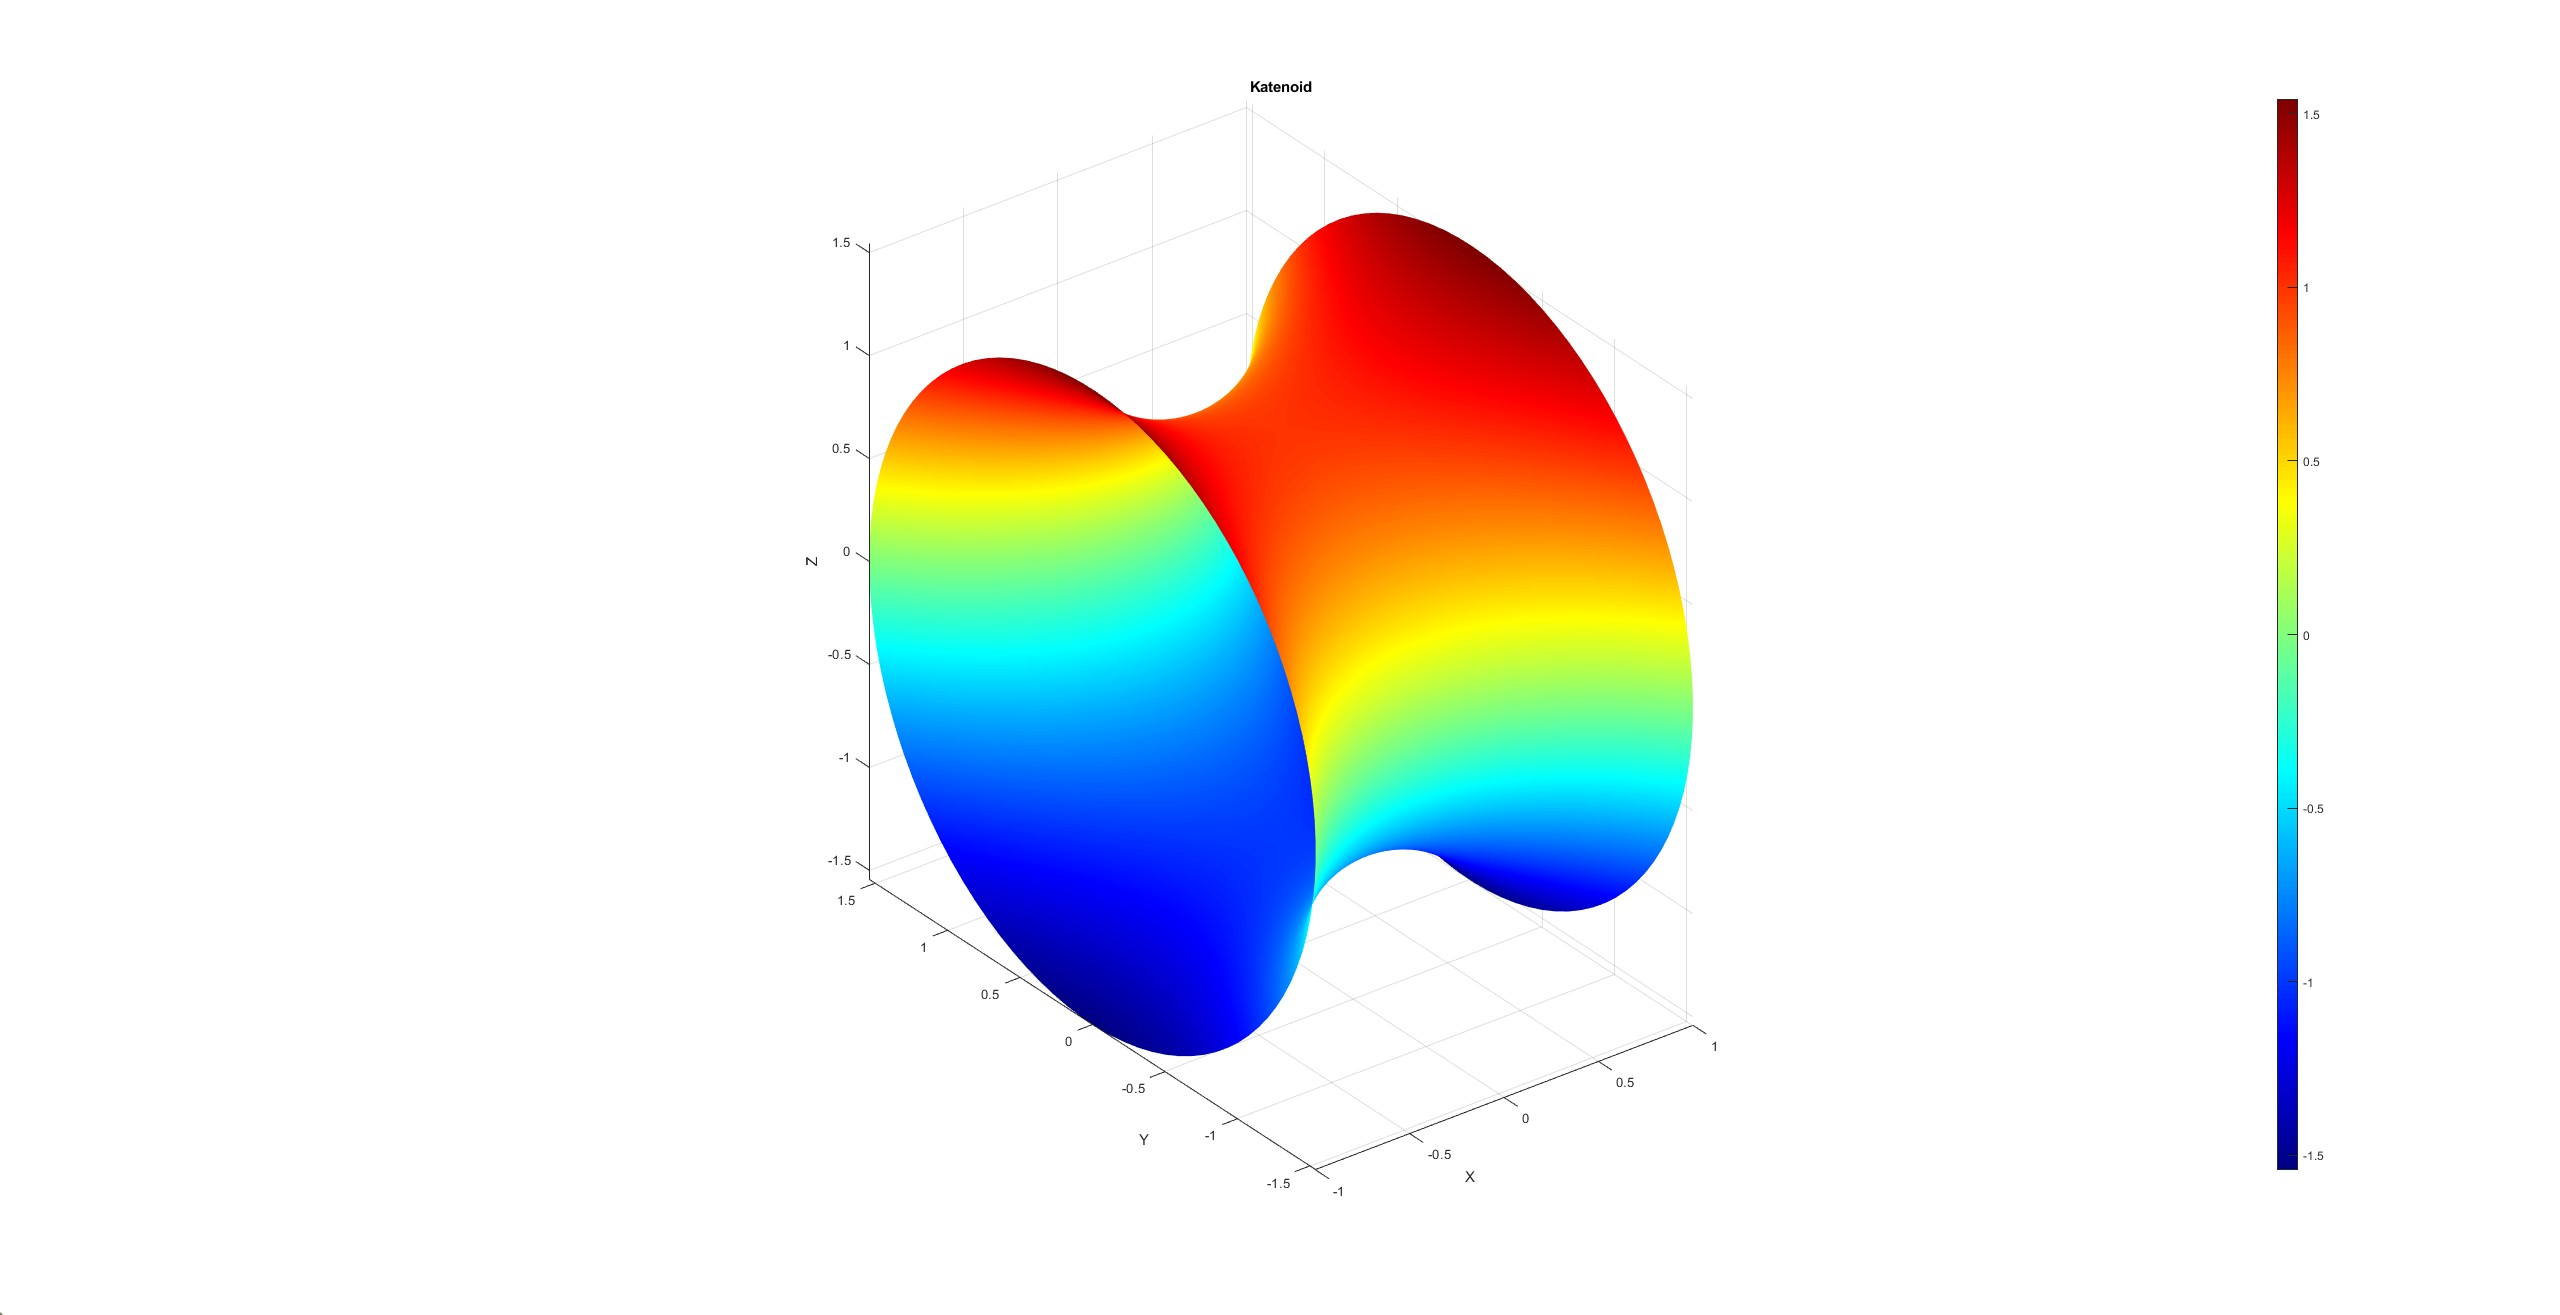
\includegraphics[width=0.7\linewidth]{papers/minimalflaechen/Katenoid}

	\caption{MATLAB Darstellung Katenoid}
	\label{fig:katenoid}
\end{figure}


\subsection{Unterschied zwischen Katenoid und Hyperboloid
	\label{Das Katenoid:subsection:Unterschied zwischen Katenoid und Hyperboloid}}
Das Katenoid (Abbildung \ref{fig:katenoid}) und das Hyperboloid (Abbildung \ref{fig:bild1}) sind beide Rotationsflächen, unterscheiden sich jedoch wesentlich in ihren geometrischen und physikalischen Eigenschaften.
Das Hyperboloid entsteht durch die Rotation einer Hyperbel und das Katenoid durch die Rotation der Kettenlinie. 
Das Katenoid ist eine Minimalfläche mit mittlerer Krümmung von Null, während das Hyperboloid eine Fläche mit konstanter negativer Krümmung ist.
Diese Unterschiede führen zu unterschiedlichen Anwendungen und strukturellen Eigenschaften.
\begin{figure}
	\centering
	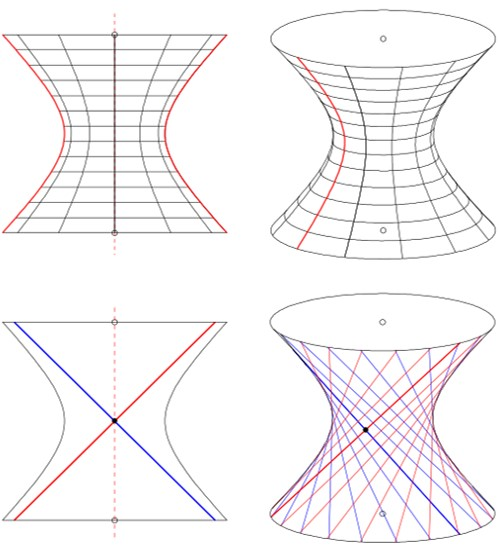
\includegraphics[width=0.7\linewidth]{papers/minimalflaechen/Bild1}
	\caption{Hyperboloid}
	\label{fig:bild1}
	\cite{minimalflaechen:Hyperboloid}
\end{figure}

